\documentclass{report}

% Title page layout and spacing configuration
% Adjust these values based on your needs
\newcommand{\vspaceone}{1cm}
\newcommand{\vspacetwo}{0.8cm}
\newcommand{\vspacethree}{1.5cm}
\newcommand{\vspacefour}{0.5cm}
\newcommand{\vspacefive}{1.0cm}
\newcommand{\vspacesix}{7cm}
\newcommand{\vspaceseven}{1cm}

% User commands and theorem styles
% If this is a group project, you can use the following commands to define the group members
% If this is individual, just add your name to both \authorname and \namelist
\newcommand{\authorname}{Group 0}
\newcommand{\namelist}{
    {Any Student (00000000)},
    {Another Student (11111111)}
}
\newcommand{\coursecode}{COMP0000J}
\newcommand{\paperdate}{\today}
\newcommand{\HRule}[1]{\rule{\linewidth}{#1}}

\newcommand{\reporttitle}{Intro to Temporal Engineering}
\newcommand{\projecttitle}{Project: A Simple Time Machine}

\begin{document}

\makenewtitlepage

% Adjust the line spacing of the contents page
\begin{spacing}{1.0}
    \tableofcontents
\end{spacing}

\newpage

% Set the title for the abstract
\renewcommand{\abstractname}{Abstract}

% Uncomment the following lines to use the colorful abstract or monochrome abstract

\begin{abstract}
    This project implements a time machine as required by \textit{COMP0000J Intro to Temporal Engineering}.
\end{abstract}

% \begin{colorfulabstract}
%     This project implements a time machine as required by \textit{COMP0000J Intro to Temporal Engineering}.
% \end{colorfulabstract}

% \begin{monochromeabstract}
%     This project implements a time machine as required by \textit{COMP0000J Intro to Temporal Engineering}.
% \end{monochromeabstract}

\section{Introduction}
    In this report, we present a simple time machine called \texttt{SIDRAT}. The time machine is a simple device that can be used to travel back in time. The time machine is powered by a flux capacitor, which generates the 1.21 gigawatts of power required to travel through time. The time machine is controlled by a simple interface that allows the user to input the desired time and date to travel to. The time machine is equipped with a safety feature that prevents the user from killing their grandparents and the creators of this machine.

\begin{figure}[ht!]
    \includegraphics[width=0.6\textwidth]{figures/placeholder.jpg}
    \caption{A placeholder image for the time machine.}
    \label{fig:placeholder}
\end{figure}


\section{Methodology}
    \subsection{Theories}
You can put your propositions, theorems and principles.
\begin{proposition}
    Time is not fixed.
\end{proposition}

\begin{theorem}
    Time travel is possible.
\end{theorem}

\begin{principle}
    Time travel is dangerous.
\end{principle}

\subsection{Notes}
There are also some predefined boxes with classical colors where you can put your notes. 
\begin{greenbox}{Green Note}
    Temporal Engineering is the study of time travel and its implications. It is a very interesting field of study. There are abundant online resources available for learning temporal engineering.
\end{greenbox}

\begin{bluebox}{Blue Note}
    You can make a lot of money after becoming a temporal engineer. The average salary of a temporal engineer is \$100,000,000 per year.
\end{bluebox}

\begin{yellowbox}{Yellow Note}
    There are many types of temporal engineer, such as frontend time machine engineer, backend time machine engineer, and full-stack time machine engineer. You can also specialize in time machine design, time machine testing, or time machine maintenance. DevOps time machine engineer is also a popular choice.
\end{yellowbox}


\section{Implementation}
    This is the implementation of the controller code of the time machine.

\begin{lstlisting}[language=Python, caption=Time Machine Demo]
def time_machine_controller():
    # This is the controller code of the time machine
    print("Time machine controller is running...")
    print("Please enter the year you want to travel to:")
    year = input()
    print(f"Travelling to {year}...")
    print("Time machine has arrived at the destination.")
    print("ERROR: Time machine has malfunctioned.")
    print("ERROR: You are now stuck in the year 2099.")
    print("ERROR: GOOD LUCK!")
\end{lstlisting}

Maybe you would like a binary tree. \par
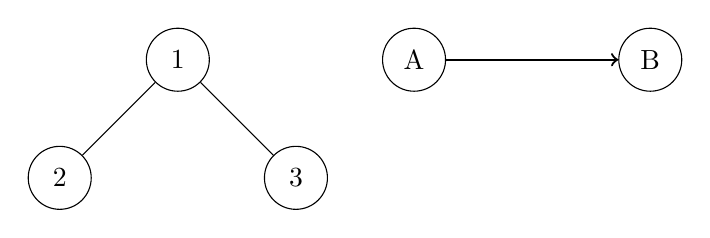
\begin{tikzpicture}[
  level distance=1.5cm,
  level 1/.style={sibling distance=3cm},
  level 2/.style={sibling distance=1.5cm},
  every node/.style={circle, draw, minimum size=0.8cm}
  ]
  \node {1}
    child {node {2}}
    child {node {3}};

  % Define nodes
  \node (A) at (3,0) {A};
  \node (B) at (6,0) {B};

  % Draw arrow from A to B
  \draw[->, thick] (A) -- (B);
\end{tikzpicture}


\section{Conclusion}
    Many people \cite{Smith_2012} believe that building a time machine is hard, but it is not impossible. In this report, we have presented a simple time machine called \texttt{SIDRAT}. We have utilized our work to change our scores in the past. Now all of us have a 4.2 GPA. It is really useful!


% Bibliography
\bibliography{bibliography/sample}
\bibliographystyle{plain}

\end{document}
